\documentclass[tikz,border=3.14mm]{standalone}
\usepackage{amsmath}

\begin{document}

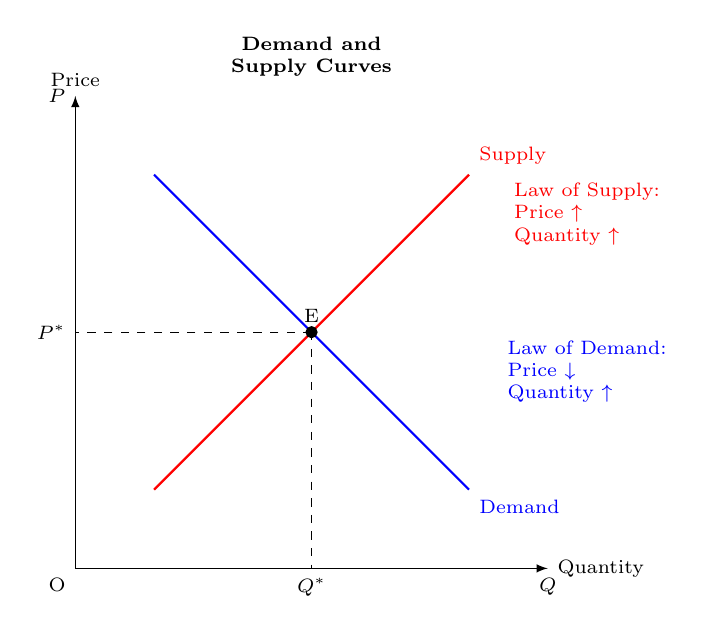
\begin{tikzpicture}[>=latex]

% Axes
\draw[->] (0, 0) -- (6, 0) node[right, font=\scriptsize] {Quantity};
\draw[->] (0, 0) -- (0, 6) node[above, font=\scriptsize] {Price};

% Labels for axes
\node[font=\scriptsize] at (0, 0) [below left] {O};
\node[font=\scriptsize] at (6, 0) [below] {$Q$};
\node[font=\scriptsize] at (0, 6) [left] {$P$};

% Demand curve
\draw[thick, blue] (1, 5) -- (5, 1) node[below right, font=\scriptsize] {Demand};

% Supply curve
\draw[thick, red] (1, 1) -- (5, 5) node[above right, font=\scriptsize] {Supply};

% Equilibrium point
\filldraw[black] (3, 3) circle (2pt) node[above, font=\scriptsize] {E};

% Dashed lines for equilibrium
\draw[dashed] (3, 3) -- (3, 0) node[below, font=\scriptsize] {$Q^*$};
\draw[dashed] (3, 3) -- (0, 3) node[left, font=\scriptsize] {$P^*$};

% Additional annotation (optional)
\node[align=center, font=\scriptsize] at (3, 6.5) {\textbf{Demand and}\\\textbf{Supply Curves}};
\node[align=left, blue, font=\scriptsize] at (6.5, 2.5) {Law of Demand: \\Price $\downarrow$ \\ Quantity $\uparrow$};
\node[align=left, red, font=\scriptsize] at (6.5, 4.5) {Law of Supply: \\Price $\uparrow$ \\ Quantity $\uparrow$};

\end{tikzpicture}

\end{document}




